\chapter{Introduction to Laravel}

Laravel เป็น Framework ของภาษา PHP สำหรับการพัฒนา Web Application 
ซึ่งพัฒนาโดย Taylor Otwell เวอร์ชันปัจจุบันคือ Laravel 8.0 
และใช้งาน Composer เพื่อจัดการ Library ที่ใช้งานทั้งหมด

\subsection{Server Requirement}
\begin{itemize}
    \item PHP >= 7.3
    \item PHP Extension: BCMath, Ctype, Fileinfo, JSON, Mbstring, OpenSSL, PDO, Tokenizer, XML
\end{itemize}

\section{การติดตั้ง Laravel Project}
1. ติดตั้ง Laravel Installer เพื่อใช้งานคำสั่ง laravel ได้ โดยใช้ terminal พิมพ์คำสั่ง
\begin{cli}{}
    composer global require laravel/installer
\end{cli}

ตรวจสอบเวอร์ชัน Laravel Installer จะได้ version 4.0.3 ซึ่งจะใช้สร้างโปรเจค Laravel version 8.0
ซึ่งเวอร์ชันอาจจะสูงกว่านี้ เนื่องจากการพัฒนาของเฟรมเวิร์คโดยตลอด
\begin{cli}{}
    laravel --version
\end{cli}

\begin{out}{}
    Laravel Installer 4.0.3
\end{out}

2. สร้างโปรเจค Laravel ชื่อ myapp ด้วยคำสั่ง laravel new myapp แล้วรอให้เสร็จสิ้น
\begin{cli}{}
    laravel new myapp
\end{cli}

\begin{out}{}
     _                               _
    | |                             | |
    | |     __ _ _ __ __ ___   _____| |
    | |    / _` | '__/ _` \ \ / / _ \ |
    | |___| (_| | | | (_| |\ V /  __/ |
    |______\__,_|_|  \__,_| \_/ \___|_|
    
    Creating a "laravel/laravel" project at "./myapp"
    Installing laravel/laravel (v8.0.1)
      - Installing laravel/laravel (v8.0.1): Downloading (100%)
    Created project in /Users/saacsos/Sites/myapp
    > @php -r "file_exists('.env') || copy('.env.example', '.env');"
    Loading composer repositories with package information
    Updating dependencies (including require-dev)

    ...
    
    Package manifest generated successfully.
    71 packages you are using are looking for funding.
    Use the `composer fund` command to find out more!
    > @php artisan key:generate --ansi
    Application key set successfully.

    Application ready! Build something amazing.
\end{out}

3. ทดสอบว่ามี Laravel Project ที่สมบูรณ์ โดยเปลี่ยน Current Directory ไปที่ myapp 
แล้วจำลอง server ด้วยคำสั่ง php artisan serve จากนั้นใช้ browser 
เข้าไปที่ http://127.0.0.1:8000 (หรือ http://localhost:8000)
\begin{cli}{}
    cd myapp
    php artisan serve
\end{cli}

\begin{out}{}
    Starting Laravel development server: http://127.0.0.1:8000
    [Sun Sep 13 12:19:24 2020] PHP 7.4.9 Development Server (http://127.0.0.1:8000) started
\end{out}

\begin{figure}[h]
    \centering
    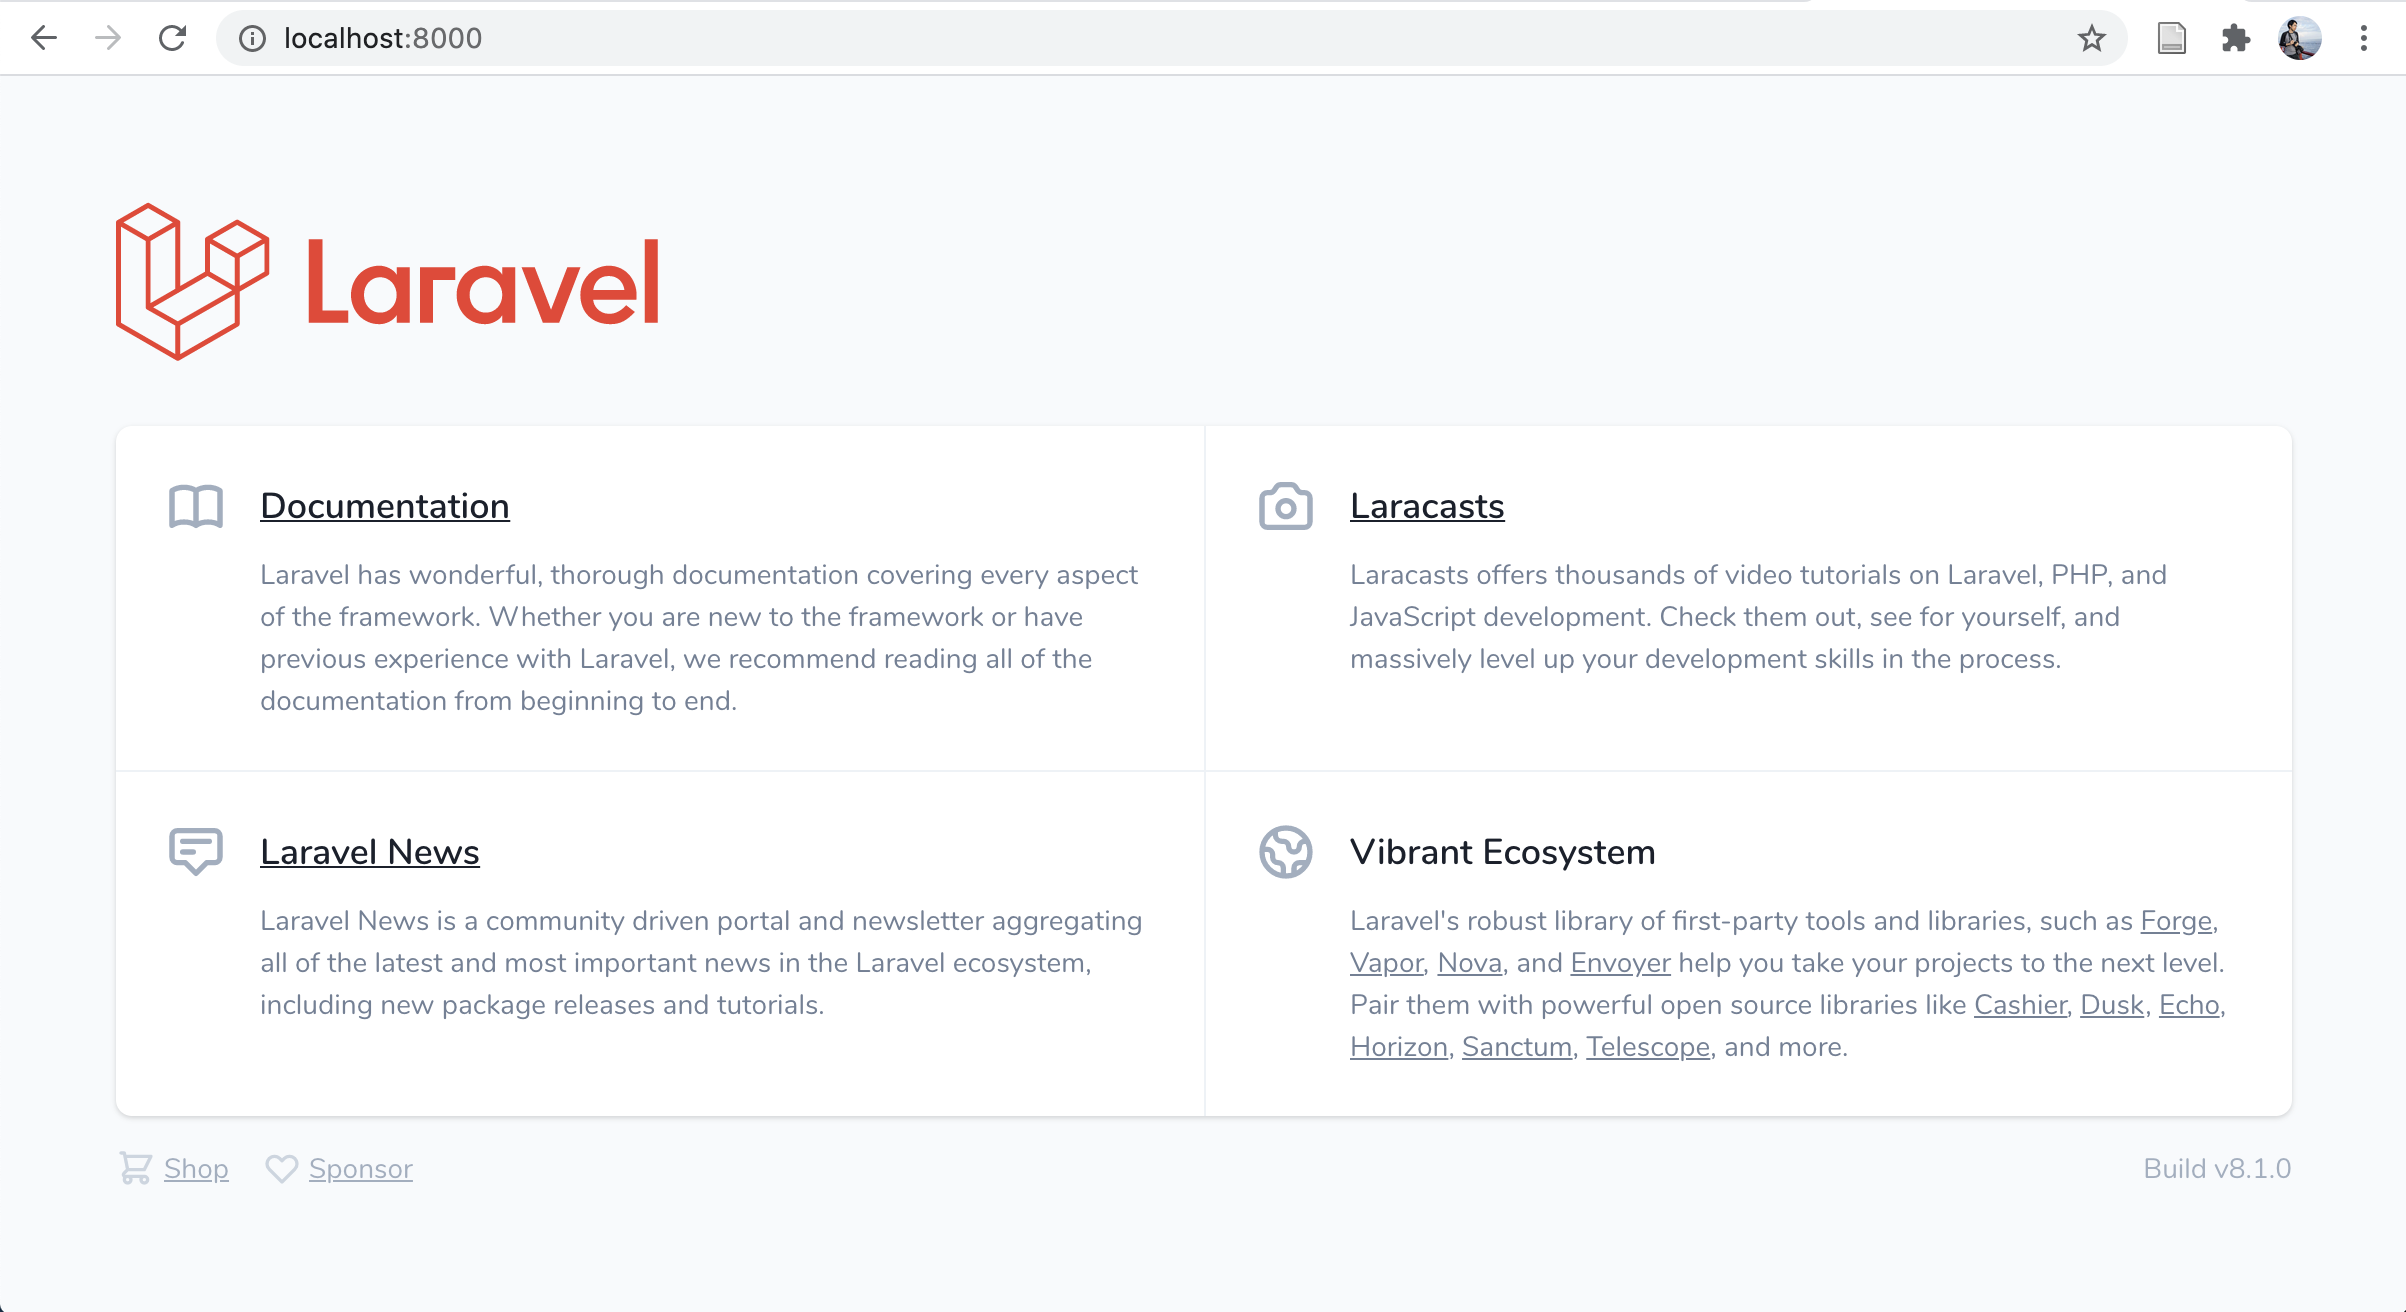
\includegraphics[width=1\textwidth]{images/ch2/01.png}
    \caption{หน้าเว็บการรันโปรเจคครั้งแรก}
\end{figure}

\subsection{ข้อควรรู้}
1. การใช้งาน Framework ตัวใดก็ตาม ควรใช้งานตาม Documentation เพื่อให้ผู้ร่วมพัฒนาเข้าใจตรงกัน
Documentation ของ Laravel Framework อยู่ที่ \href{https://laravel.com/docs/}{https://laravel.com/docs/}

2. Framework เกิดจากการทำงานของไลบรารี่หลายตัวร่วมกัน ข้อผิดพลาดส่วนใหญ่เกิดจากการเขียนโค้ดผิด 
หรือส่งค่าไปเรียกฟังก์ชันผิด ซึ่งข้อผิดพลาดที่แสดงนั้นมักจะบอกว่าเกิดขึ้นในไฟล์ที่เราไม่ได้สร้าง 
ดังนั้นอย่าลบไฟล์หรือแก้ไขไฟล์ที่ตนเองไม่ได้สร้างเด็ดขาด ควรหาข้อมูลก่อนว่าข้อผิดพลาดเกิดขึ้นจากอะไร 
เป็นเพราะเขียนโค้ดผิดหรือไม่ หรือเป็นเพราะส่งค่าผิด

3. การ Deploy Laravel Project ให้แก้ไข .env file โดยเปลี่ยน \mintinline{console}{APP_ENV=production} 
และ \mintinline{console}{APP_DEBUG=false} การตั้งค่าต่าง ๆ ควรตั้งค่าที่ .env file เท่านั้น

4. ไม่ควร push .env file ขึ้น git server

5. Laravel Project ที่ clone จาก git server ก่อนจะพัฒนาต่อ ให้สั่ง
\begin{cli}{}
    composer install
    composer dump-autoload
\end{cli}

6. กำหนด Document Root มาที่ Directory public/ เพื่อไม่ให้เข้าถึงโค้ด
\begin{code}{apache}{ตัวอย่างการตั้งค่าของโปรเจคใน Apache Server}{}
    <VirtualHost *:80> 
        DocumentRoot "C:/laragon/www/myapp/public/"
        ServerName myapp.test
        ServerAlias *.myapp.test
        <Directory "C:/laragon/www/myapp/public/">
            AllowOverride All
            Require all granted
        </Directory>
    </VirtualHost>
\end{code}

\subsection{การตั้งค่าเริ่มต้นของ Laravel Project}
การตั้งค่าต่าง ๆ มักจะกำหนดในไฟล์ \mintinline{bash}{.env} เป็นส่วนใหญ่ เช่น การเชื่อมต่อฐานข้อมูล 
การตั้งค่า Mail Driver การตั้งค่า Session แต่มีการตั้งค่าบางส่วนที่ต้องไปแก้ไขในไฟล์ 
\mintinline{bash}{config/app.php} ดังนี้
\begin{itemize}
    \item \mintinline{php}{timezone} กำหนดเป็น \mintinline{php}{Asia/Bangkok}
    \item \mintinline{php}{provider} หากมีการสร้าง Provider ขึ้นเอง
    \item \mintinline{php}{alias} หากต้องการกำหนด Facade ของ Class
\end{itemize}